\documentclass[a4paper, oneside]{article}
\usepackage{array}
\usepackage{shortvrb}
\usepackage{listings}
\usepackage{fullpage}
\usepackage{enumerate}
\usepackage{graphicx}
\usepackage{subfigure}
\usepackage{url}
\usepackage{indentfirst}
\usepackage{eurosym}
\usepackage{listings}
\usepackage{color}
\usepackage{fancybox}
\usepackage{ulem}
\usepackage{wrapfig}
\usepackage{systeme}
\usepackage{tabularx}
\usepackage{subfig}
\usepackage[dvipsnames]{xcolor}



\begin{document}
\begin{titlepage}
	\newcommand{\HRule}{\rule{\linewidth}{0.5mm}}
	\center
	\textsc{\LARGE Université de Liège}\\[1cm]
	\textsc{\Large Faculté des Sciences Appliquées}\\[2cm]
		
	\HRule \\[0.5cm]
	{ \huge \bfseries Automatic Multispeaker Voice Cloning Across Languages}\\[0.2cm]
	\HRule \\[3cm]

	\begin{minipage}{0.4\textwidth}
		\begin{flushleft} \Large
			\emph{Author:}\\
			Corentin \textsc{Jemine}
		\end{flushleft}
	\end{minipage}
	~
	\begin{minipage}{0.4\textwidth}
		\begin{flushright} \Large
			\emph{Supervisor:} \\
			Prof. Gilles \textsc{Louppe}
		\end{flushright}
	\end{minipage}\\[4cm]
	
	{\LARGE Academic year 2018 - 2019}\\[2cm]
	
	
\includegraphics{images/uliege_logo.jpg}\\[1.25cm]
	
	\textit{Graduation studies conducted for obtaining the Master's degree \\in Data Science by Corentin Jemine}
	
	\vfill
\end{titlepage}

\setcounter{page}{2}

\section{Abstract}
\color{red}
To do when I'll have a good overview of the project. Try to answer:
\begin{itemize}
	\item What is the goal of the application? What are its requirements, what is the setting, what kind of data are we going to use it on?
	\item What is zero-shot voice cloning? How does it fit in here (difference between an online and offline approach)?
	\item What are the particularities of our implementation (both model and datasets), what are its upsides and downsides (for example: requires huge datasets but fast inference)?
	\item What did we ultimately achieve? How good are our results?
\end{itemize}
\color{black}

\section{Introduction}

\color{red}
Concise presentation of the problem

Processing of text into features

Present the generic framework of SPSS since it doesn't change much over the years?

SOTA ON MULTISPEAKER TTS:

\color{black}
Previous state of the art \color{red} is it really sota when concatenative often leads to more natural results? to review \color{black} in TTS include hidden Markov models (HMM) based speech synthesis, which is a statistical parametric speech synthesis (SPSS) method. HMMs learn a distribution over mel-frequency cepstral coefficients (MFCC) with energy, their delta and delta-delta coefficients \cite{TTSSOTA}. These speech parameters are derived from their distribution by maximum likelihood before going through a vocoder such as MLSA \cite{MLSA}. The input text to generate is processed into a sequence of linguistic contexts. The HMM parameters to use for speech generation are distributed conditionally to these contexts. Indeed, contexts are clustered with decision trees and an HMM is learned for each cluster \cite{HMMTTS} (effectively partitioning the training set). It is possible to modify the voice generated by conditioning on a speaker or tuning these parameters with adaptation or interpolation techniques (e.g. \cite{HMMSpeakerInterpolation}  \color{red} elaborate a bit on these techniques? \color{black}), making HMM-based speech synthesis a multispeaker TTS system. \color{red} Compare with concatenative? see \cite{SPSSDNN} and https://ieeexplore.ieee.org/document/541110 \color{black}

\begin{wrapfigure}{r}{7cm}
	\vspace{-0.6cm}
	\centering
	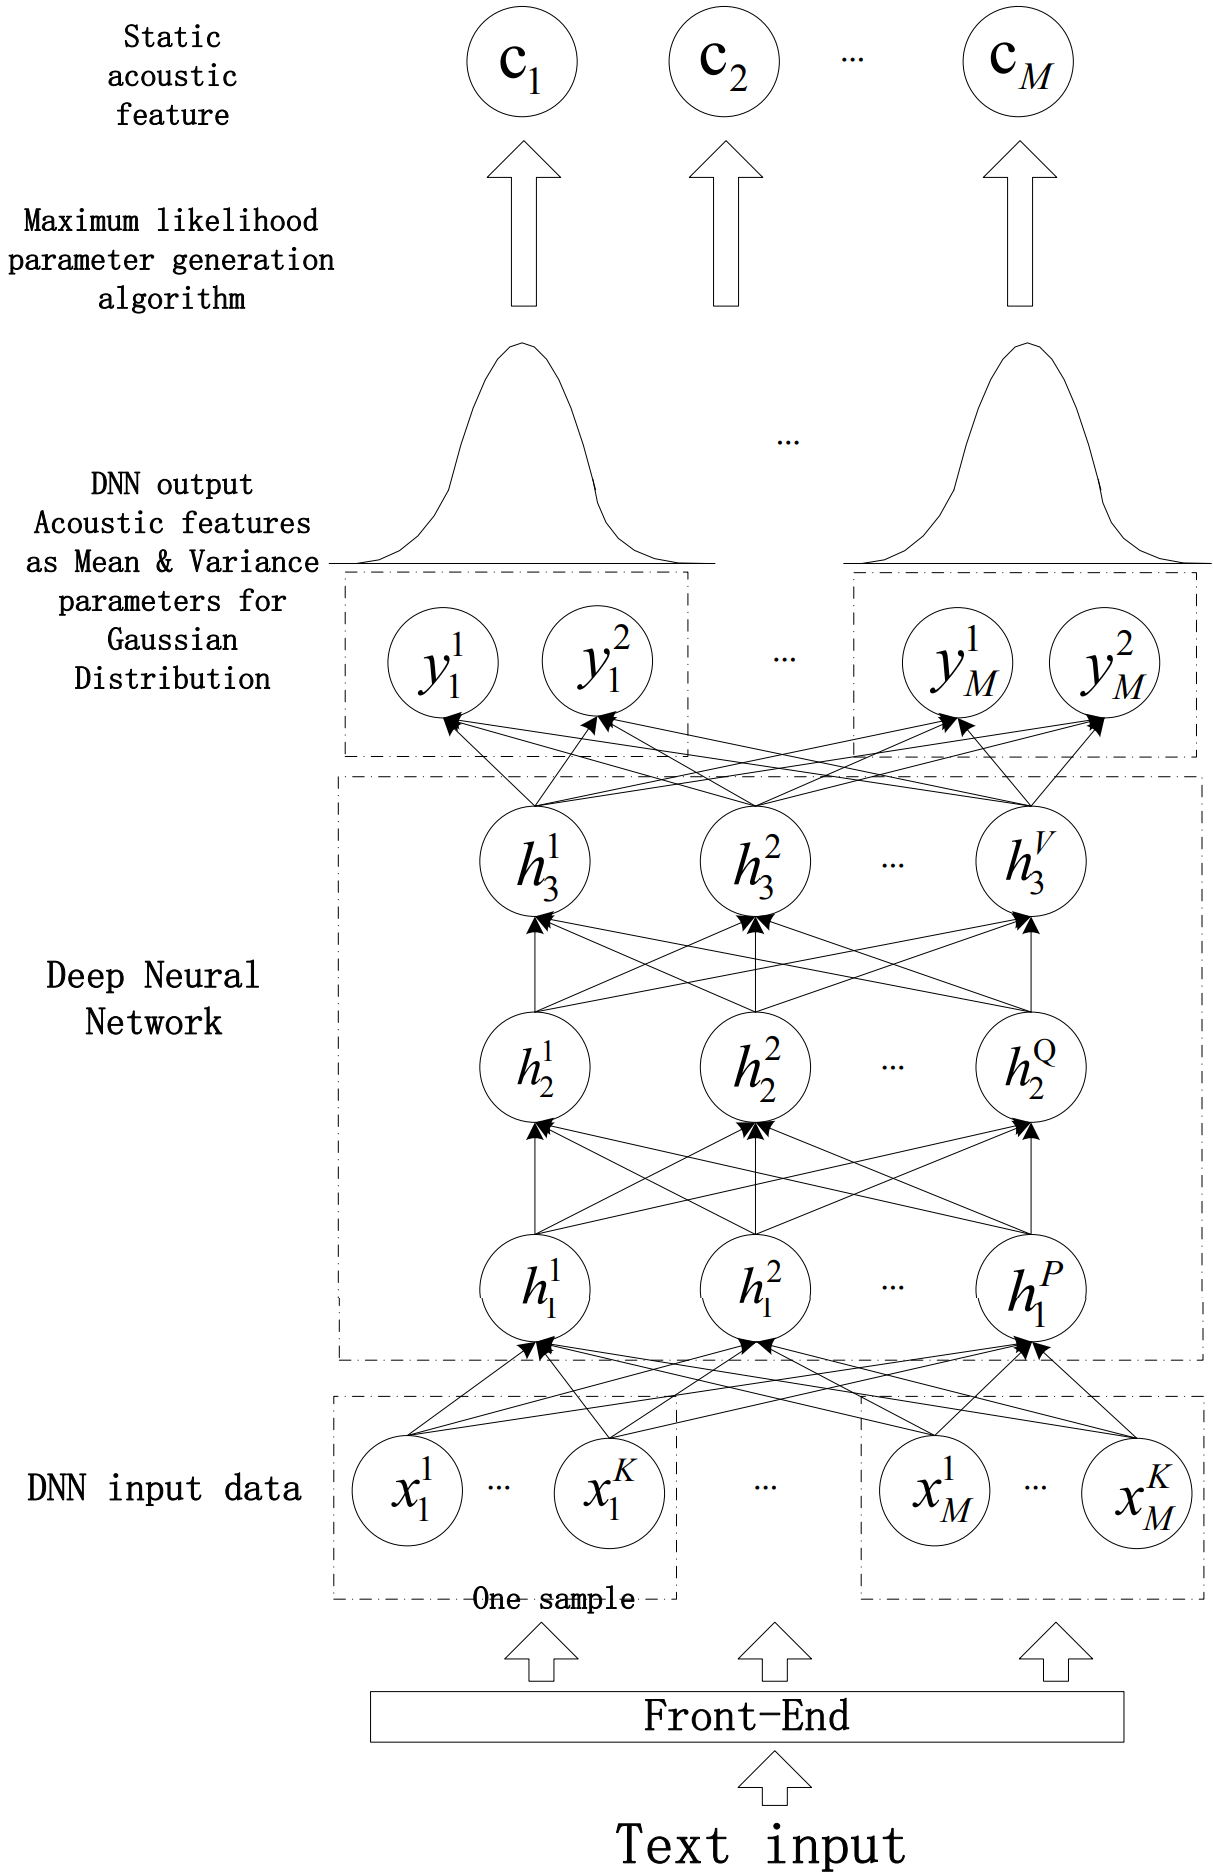
\includegraphics[width=7cm]{images/dnn_spss.png}
	\caption{caption}
	\label{label}
	\vspace{-1.1cm}
\end{wrapfigure}

Improvements to this framework were later brought by feed-forward and recurrent deep neural networks (DNN and RNN respectively) as a result of progress in both hardware and software. \cite{SPSSDNN} proposes to replace entirely the decision tree-clustered HMMs in favor of a DNN. They argue for better data efficiency as the training set is no longer fragmented in different clusters of contexts. They demonstrate improvement over the speech quality with a similar number of parameters as in the HMM-based approach.


\color{blue}
Several authors propose to replace the decision trees by a DNN, arguing for better data efficiency and for more representational power of complex dependencies \cite{Hashimoto-2015, Lu_combininga, 6854318, Yin2014ModelingDP}. Most demonstrate improved speech quality for a similar number of parameters \cite{Hashimoto-2015, 6854318, Yin2014ModelingDP}.
\color{black}

\color{red} Entirely read \cite{Hashimoto-2015} if missing infos about HMMs + DNNs \color{black}


\color{red}


Wavenet:

Breakthrough in TTS with raw waveform gen

Take images from https://deepmind.com/blog/wavenet-generative-model-raw-audio/ ?

Dilated causal convolutions

Condition on a speaker identity

Tacotron

Deep voice (1, 2, 3 + few samples), Tacotron 2

SV2TTS

Extensions?
\color{black}



\color{red}
\color{black}

\clearpage
\bibliographystyle{plain}
\bibliography{references} 




















%$$\Leftrightarrow h_b(x) =
%\left\{\begin{array}{lll}
%0 & if & P(y = 0 | x) > P(y = 1 | x)\\ 
%1 & else &
%\end{array}\right.$$



%\begin{figure}[h]
%	\centering
%	\includegraphics[width=16cm]{image.png}
%	\caption{caption}
%	\label{label}
%\end{figure}



%\begin{figure}[h]
%	\centering
%	\captionsetup{justification=centering}
%	\hspace{-1cm}
%	\subfigure{\includegraphics[height=5cm]{image.png}}
%	\subfigure{\includegraphics[height=5cm]{image.png}}
%	\hspace{-1cm}
%	\caption{caption}
%	\label{label}
%\end{figure}


%\begin{center}
%	\begin{tabular}{|r|ccc|ccc|}
%		\hline
%		& \multicolumn{6}{c|}{Validation set}\\
%		\hline
%		& \multicolumn{3}{c|}{Valid images (3126)} & \multicolumn{3}{c|}{Invalid images (3126)} \\
%		\hline
%		& Correct & Unclassified & Incorrect & Correct & Unclassified & Incorrect \\
%		\hline
%		Reduced & 94.98\% & 3.07\% & 1.95\% & 95.27\% & 2.91\% & 1.82\% \\
%		Lenet & 98.08\% & 0.74\% & 1.18\% & 97.86\% & 0.96\% & 1.18\% \\
%		\hline
%	\end{tabular}
%	
%	\vspace{0.5cm}
%	  
%	\begin{tabular}{|r|ccc|ccc|}
%		\hline
%		& \multicolumn{6}{c|}{Test set}\\
%		\hline
%		& \multicolumn{3}{c|}{Valid images (999)} & \multicolumn{3}{c|}{Invalid images (74)} \\
%		\hline
%		& Correct & Unclassified & Incorrect & Correct & Unclassified & Incorrect \\
%		\hline
%		Reduced& 94.29\% & 3.70\% & 2.00\% & 95.95\% & 4.05\% & 0.00\%  \\
%		Lenet & 96.90\% & 1.30\% & 1.80\% & 97.30\% & 1.35\% & 1.35\% \\
%		\hline
%	\end{tabular}
%\end{center}


\end{document}













































































































